\documentclass[aspectratio=169]{beamer}
\beamertemplatenavigationsymbolsempty

\mode<presentation>
{
	\usetheme{Singapore}
	\setbeamercovered{transparent}
	\setbeamertemplate{footline}[frame number]
}

% \usepackage{flashmovie}
\usepackage[utf8]{inputenc}
\usepackage[T1]{fontenc}
%\usepackage[ngerman]{babel}
\usepackage[english]{babel}
\usepackage{amsmath}
\usepackage[absolute,overlay]{textpos}

\usebackgroundtemplate{%
\begin{tikzpicture}[remember picture,overlay]
\node[anchor=south west] at (current page.south west) {\includegraphics[height=0.4cm]{by.eps}};
\end{tikzpicture}}

\author{Anton Kuzmin}

\institute[]
{
%	Informatik 3 / Rechnerarchitektur\\
%	Universität Erlangen Nürnberg
}
\date{@DATE@}

\usepackage{tikz}

\title{On-hardware debugging of IP cores with free tools}

\setbeamerfont{table font}{size=\tiny}

\begin{document}

\begin{frame}
  \titlepage
\end{frame}

\section{Intro}

\begin{frame}
  \frametitle{Who am I\dots}
  \begin{itemize}
  \item not really a software developer\\
    \dots but write code sometimes
  \item developing embedded systems for 25 years
  \item VME, CompactPCI, AdvancedTCA, SoM
  \item FPGA and SoC-FPGA (Altera/Intel, Microsemi/Microchip)
  \item VHDL (RTL-code, no, it is not a software)
  \end{itemize}
  \vskip.5cm

  My usual problem with the software is how to make it run on a
  hardware which is known not to be working yet and how to bring-up
  and test this hardware. With a soft-core CPU it is getting even
  worse.

\end{frame}


\frame{\tableofcontents[subsectionstyle=show]}

\section{Why FPGA (and what the FPGA is all about)}

\begin{frame}
\frametitle{Why software develpers should care about FPGA}
\begin{itemize}
  \item conventional hardware architectures are stuck
  \item the only two mainstream HDLs represent software technology
  level of a stone age (well, last century)
\end{itemize}
\vskip.5cm
Therefore\dots
\vskip.5cm
\begin{itemize}
  \item you need it to make next generation software run on
  heterogeneous and malleable hardware
  \item industry needs your help to move forward
\end{itemize}
\end{frame}

\section{Software approach -- simulation first}

\begin{frame}
\frametitle{Free software for HDL developers}
\textbf{Simulate it!!}
\begin{itemize}
  \item Verilog HDL
  \begin{itemize}
    \item Verilator (\texttt{https://www.veripool.org/wiki/verilator})
    \item Icarus Verilog (\texttt{http://iverilog.icarus.com/})
    \item Yosys (\texttt{http://www.clifford.at/yosys/})
  \end{itemize}
  \item VHDL: \textbf{\texttt{ghdl}} (\texttt{http://ghdl.free.fr/})\\
  GHDL is an open-source simulator for the VHDL language.
  \item GTKWave (\texttt{http://gtkwave.sourceforge.net/})\\
  GTKWave is a fully featured cross-platform wave viewer
\end{itemize}
Unit and regression testing for hardware blocks (Python cocotb, VPI, etc.)
\end{frame}

\begin{frame}[fragile]
\frametitle{VHDL code snippet}
\begin{verbatim}
  process (d, mode)
  begin
    if mode = '0' then
      d_next <= std_logic_vector(unsigned(d) + 1);
    else
      d_next(7 downto 1) <= d(6 downto 0);
      d_next(0) <= d(7) xor d(5) xor d(4) xor d(3);
    end if;
  end process;
\end{verbatim}
\end{frame}

\begin{frame}
  \frametitle{GTKWave with GHDL simulation results}
  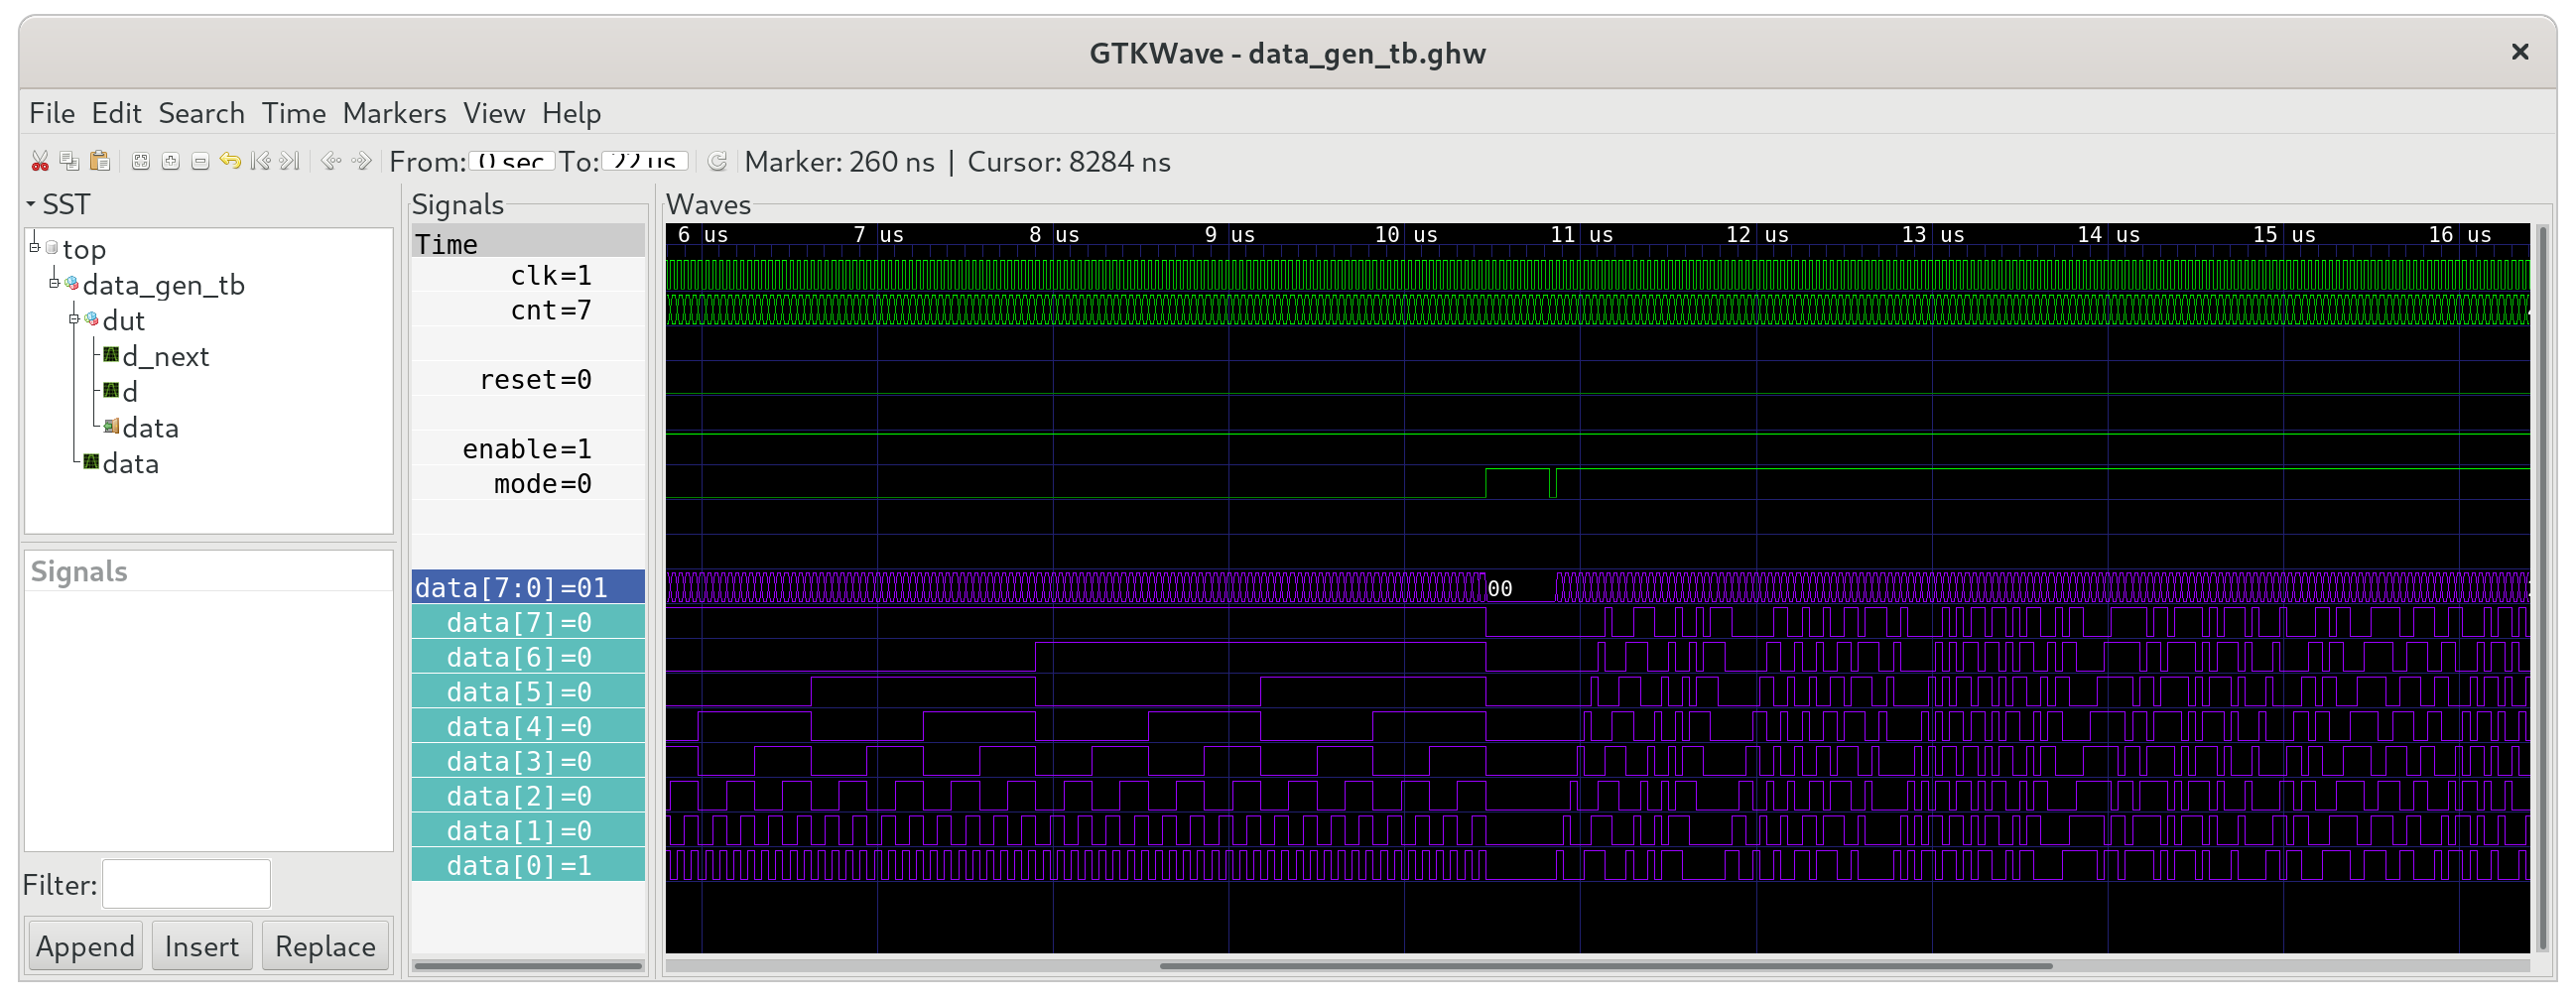
\includegraphics[width=\textwidth]{sim.png}
  \dots and live demo
\end{frame}

\section{Going to the hardware}

\begin{frame}
\frametitle{On-chip instrumentation}
Proprietary and vendor specific tools (and their problems)
\begin{itemize}
  \item Altera/Intel SignalTAP
  \item Xilinx ChipScope
  \item Synopsys Identify RTL Debugger
  \item Microsemi/Microchip SmartDebug
\end{itemize}
What is in common: standard inteface to the hardware IEEE 1149.1
(JTAG)
\end{frame}

\begin{frame}
\frametitle{Assembling a puzzle}
\begin{itemize}
  \item Free software to speak with hardware on IEEE-1149.1
  \begin{itemize}
    \item UrJTAG (\texttt{http://urjtag.org/})
    \item OpenOCD (\texttt{http://openocd.org/})
  \end{itemize}
  \item libsigrok (\texttt{https://sigrok.org/})
  \item PulseView (sigrok Logic Analyzer GUI)
  \item SpiderBoard with SpiderSoM
  (\texttt{http://www.spiderboard.org/})\\
  or MX10 (\texttt{https://www.aries-embedded.com/system-on-module/fpga/})\\
  Altera/Intel MAX10 FPGA module with built-in USB-to-JTAG interface
\end{itemize}
\end{frame}

\begin{frame}
  \frametitle{Logic Analyzer trace}
  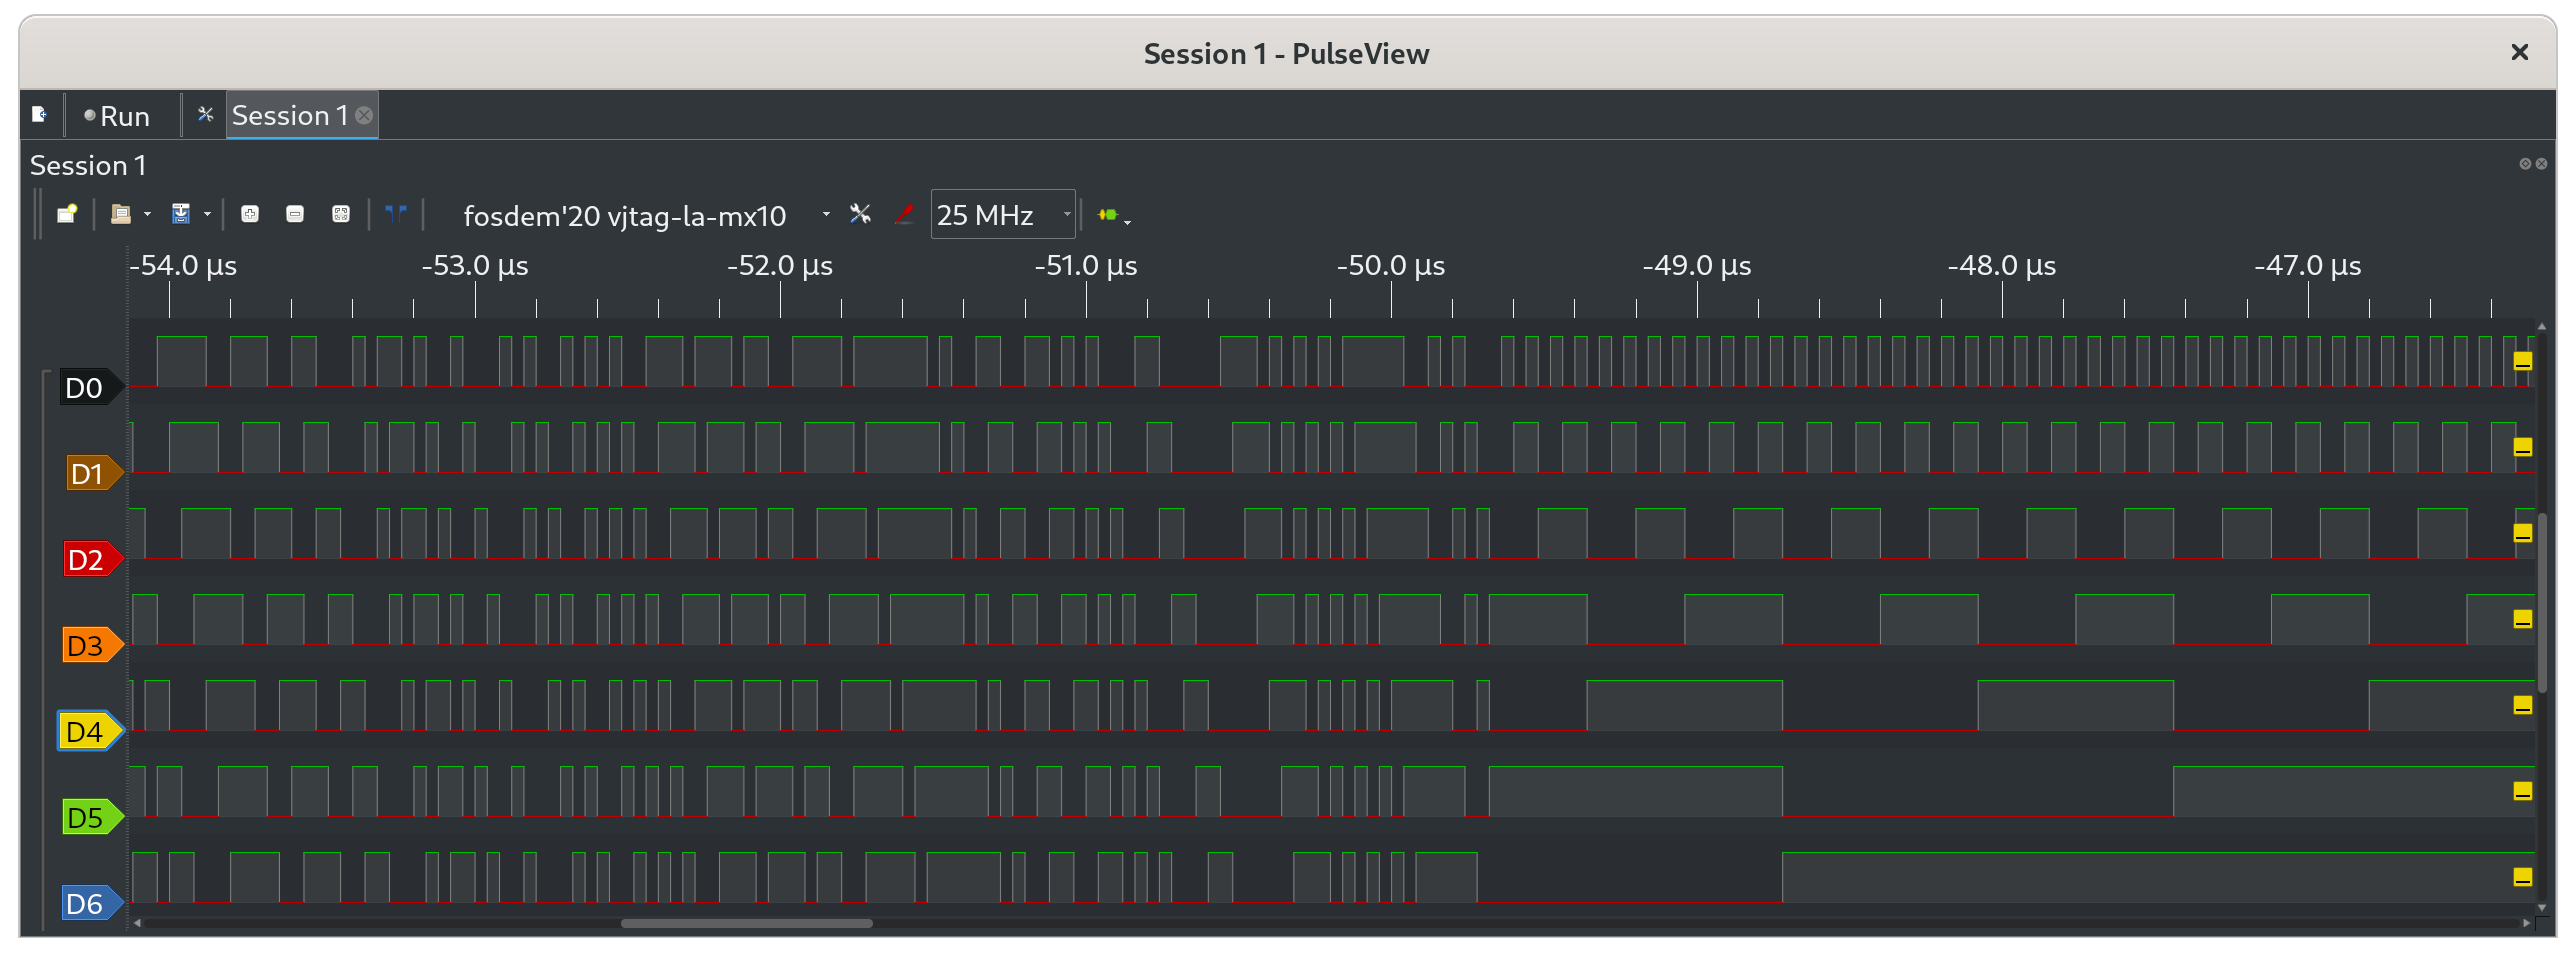
\includegraphics[width=\textwidth]{pulseview.png}
  \dots and live demo
\end{frame}

\section{What's next}

\begin{frame}
\frametitle{Challenges ahead}
\begin{itemize}
  \item \textbf{integration}
  \item support for different hardware interfaces, FPGA vendors,
  device families
  \item automated design instrumentation (kudos to vendor tools)
  \item IEEE-1149.7, IEEE-1687 (2014), etc.
  \item integration with software debugging tools
\end{itemize}
\end{frame}

\section{Contact info}
\begin{frame}

  \begin{minipage}{7cm}
    \vskip.5cm
    \huge{Thank you!}
    \vskip1cm
    \small{Anton Kuzmin}\\
    \small{\texttt{anton.kuzmin@cs.fau.de}}\\
    \small{\texttt{https://github.com/ak-fau/}}
    \vskip.5cm
    \Huge{Questions?..}
  \end{minipage}

  \vspace{-5cm}
  \begin{flushright}
    \includegraphics[height=5cm]{github-vcard.png}\\
  \end{flushright}

\end{frame}


\end{document}
